\section{Deep Q Networks}
\label{sec:DQN}
The first deep reinforcement learning network there has been created in this project is the Deep Q Network. The Deep Q Network was first time described in the paper "playing Atari with Deep reinforcement learning" \cite{DBLP:journals/corr/MnihKSGAWR13} published by DeepMind. In this paper they learned the computer to play Atari 2600 video games. The computer only observed the screen pixels from the game, and received a reward when the game score increased. The result was remarkable, because the games and the goals in the games are very different. The same architecture was used for seven different games. In 3 of the seven games the computer performed better than the best human. 

To understand the problem the Deep Q Network solved, it is easier to use an example, here we use the game Breakout as an example. In this game you control a paddle at the bottom of the screen, and have to clear the bricks in the top of the screen. This is done by bouncing a ball between the paddle and the bricks. Each time a brick is hit it disappears and the game score increases. The game can be seen on figure \Cref{fig:Atari_breakout}

\begin{figure}[H]
	\centering
	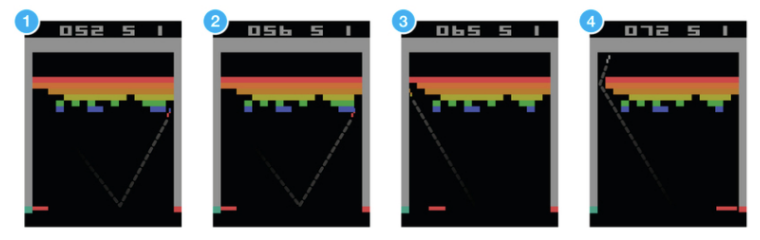
\includegraphics[width=1\textwidth]{Figures/Architecture/DQN/Atari_breakout.png}
	\caption{Atari Breakout game. Image credit: DeepMind\cite{DBLP:journals/corr/MnihKSGAWR13} }
	\label{fig:Atari_breakout}
\end{figure}

To teach a Network how to play this game, the input to the network is the screen images, and the output is the actions of the game: left, right or fire (to launch the ball). One approach to this problem is to treat it as a classification problem - for each screen decide if the paddle should move left, right or press fire. To do this lots of training examples is needed. The problem about this approach is thats really how human learns, we don't need someone to tell us million times which move to choose at each screen. Instead human just need occasional feedback that we did the right thing, and then learn from it ourself. This is the task reinforcement learning tries to solve, more of the reinforcement learning theory can be read in \textbf{Reference to Theory chapter}.

While the idea is quite intuitive, in practice there are numerous challenges. One of the challenges is when hitting a brick and the reward is received, it often has nothing to do with the actions (paddle movement) just before the reward was received. All the work was done when the paddle was positioned correctly and bounced the ball back. This is called the credit assignment problem – i.e., which of the preceding actions was responsible for getting the reward and to what extent.

Another challenge is when a strategy is found and a certain reward is received, should the program stick with that strategy or experiment with something that could lead to a bigger reward. This is called the explore-exploit dilemma – should you exploit the known working strategy or explore other, possibly better strategies. 

The screen pixels obtain most of the relevant information of the game situation, except speed and direction of the ball. This could be covered by having two consecutive screens. 

\subsection{Preprocessing}
The DeepMind paper use preprocessing where the take the last four screen images, resize them to 84x84 and convert to grayscale with 256 gray levels. This will give $256^{84x84x4} \approx 10^{67970}$ possible game states. This will give $10^{67970}$ rows in the imaginary Q-table - more than the number of atoms in the universe. Many pixel combinations never occur, so possible represent it as a sparse table containing only visited states. Most of the states are rarely visited and it would take a lifetime of the universe to the q-table to converge. It should also be possible to have a good guess for Q-values for states we have never seen. 

To do this deep learning comes in to the picture. Neural networks are extremely good at coming up with good features for highly structured data. A way neural networks can be used in reinforcement learning is it could represent the Q-function, where it takes the state (four game screens) and action as an input and output the corresponding Q-value. Another way is to only take game screens as input, and output the Q-value for each possible action. The second approach has the advantages, that if we want to perform a Q-value update or choose the action with the highest Q-value, it can be done by only doing one forward pass in the network and have all Q-values for all possible actions. The two different approaches to use neural network to represent the Q-function can be seen on \Cref{fig:DQN_two_approach}.              


\begin{figure}[H]
	\centering
	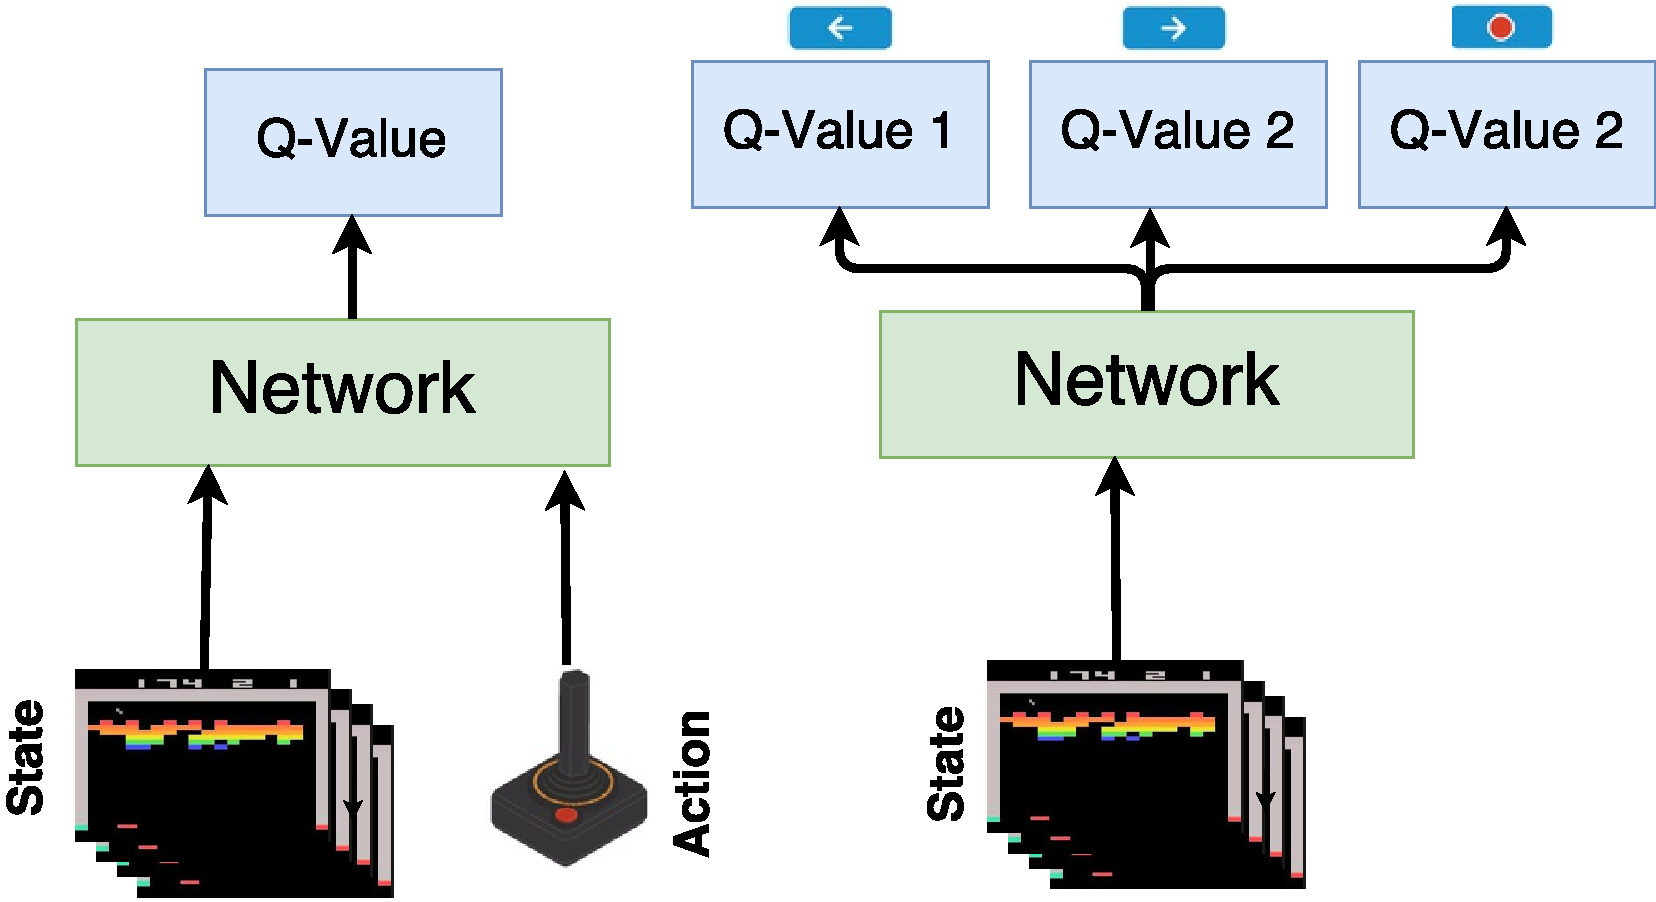
\includegraphics[width=1\textwidth]{Figures/Architecture/DQN/DQN_two_approach.pdf}
	\caption{Left: Naive formulation of deep Q-network. Right: More optimized architecture of deep Q-network, used in DeepMind paper.} 
	\label{fig:DQN_two_approach}
\end{figure}    

The network architecture that DeepMind used can be seen on the table below \Cref{tab:DQN_network}. 

\begin{table}[H]
	\centering
	\caption{Architecture of the Deep Q Network used by DeepMind}
	\label{tab:DQN_network}
	\begin{tabular}{|l|c|c|c|c|c|c|}
		\hline
		\rowcolor[HTML]{9B9B9B} 
		\multicolumn{1}{|c|}{\cellcolor[HTML]{9B9B9B}\textbf{Layer}} & \textbf{Input} & \textbf{Filter size} & \textbf{Stride} & \textbf{Num filters} & \textbf{Activation} & \textbf{Output} \\ \hline
		\cellcolor[HTML]{FFFFFF}\textbf{conv1}                       & 84x84x4        & 8x8                  & 4               & 32                   & ReLU                & 20x20x32        \\ \hline
		\rowcolor[HTML]{C0C0C0} 
		\textbf{conv2}                                               & 20x20x32       & 4x4                  & 2               & 64                   & ReLU                & 9x9x64          \\ \hline
		\cellcolor[HTML]{FFFFFF}\textbf{conv3}                       & 9x9x64         & 3x3                  & 1               & 64                   & ReLU                & 7x7x64          \\ \hline
		\rowcolor[HTML]{C0C0C0} 
		\textbf{fc4}                                                 & 7x7x64         &                      &                 & 512                  & ReLU                & 512             \\ \hline
		\cellcolor[HTML]{FFFFFF}\textbf{fc5}                         & 512            &                      &                 & 18                   & Linear              & 18              \\ \hline
	\end{tabular}
\end{table}


        